
\subsubsection{04.11.14}

\begin{enumerate}
	\item Время начала и окончания собрания:\newline
	14:00 – 20:30
	\item Цели собрания:\newline
	\begin{enumerate}
	  \item	Переделать конструкцию лебедки.\newline
	  
	  \item	Подсоединить энкодер к одному из приводов лебедки.\newline
	  
	  \item	Добавить в программу управления лебедкой ограничения ее движения.\newline
	  
    \end{enumerate}
    
	\item Проделанная работа:\newline
	\begin{enumerate}
	  \item	Механизм лебедки был изменен в соответствии с идеями, выдвинутыми на предыдущем занятии.\newline
      
      \item	Энкодер был установлен на левый привод лебедки.\newline
      
      \begin{figure}[H]
      	\begin{minipage}[h]{0.5\linewidth}
      		\center{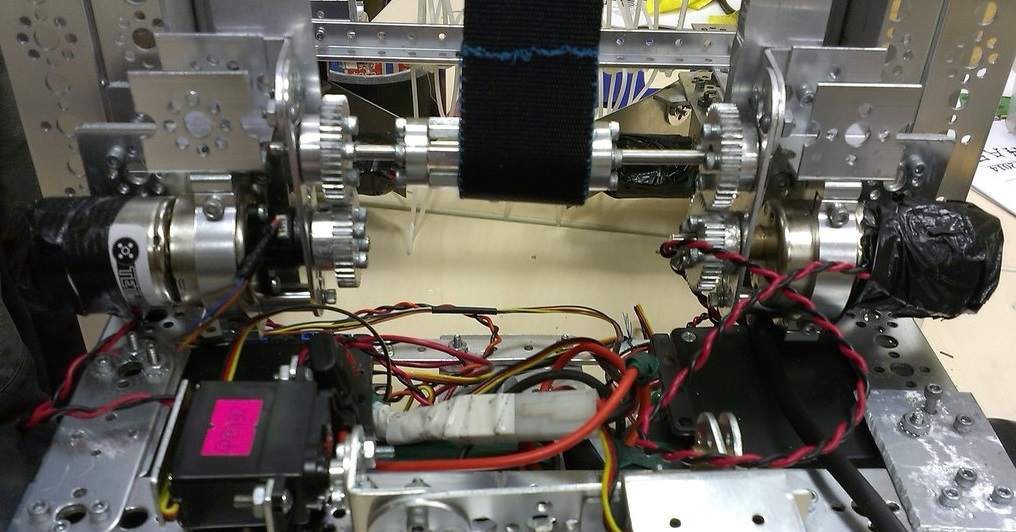
\includegraphics[width=1\linewidth]{days/04.11.14/images/01}}
      		\caption{Окончательная версия механизма лебедки}
      	\end{minipage}
      	\hfill
      	\begin{minipage}[h]{0.5\linewidth}
      		\center{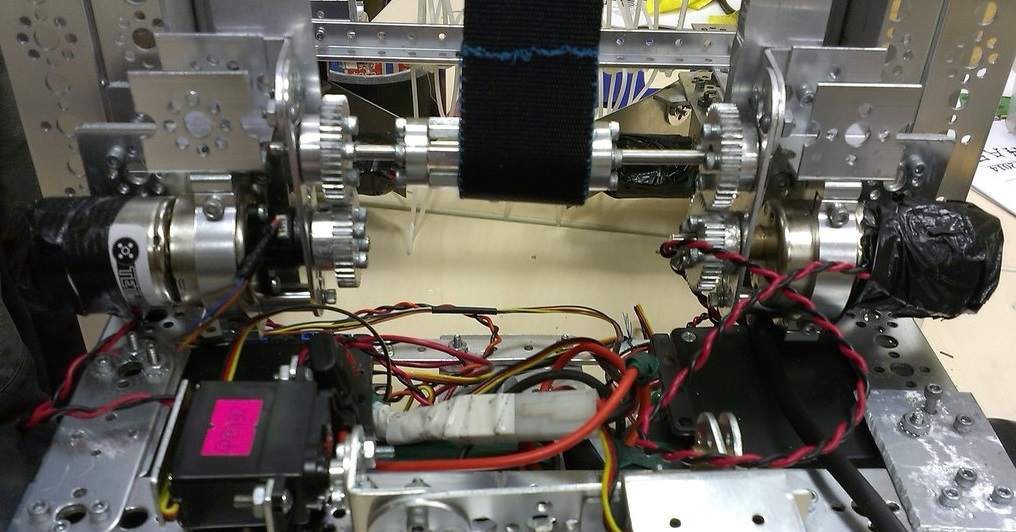
\includegraphics[width=1\linewidth]{days/04.11.14/images/01}}
      		\caption{Энкодер}
      	\end{minipage}
      \end{figure}
      
      \item	В программу были добавлены ограничения движения лебедки. Таким образом, если показания энкодера превышали допустимое значение, лебедка автоматически останавливалась.\newline
      
      \item	Испытания лебедки прошли успешно. Новая конструкция лебедки была надежна и не имела никаких проблем с раздвиганием подъемника.\newline
      
    \end{enumerate}
    
	\item Итоги собрания: \newline
	\begin{enumerate}
	  \item	Работа над механизмом лебедки завершена.\newline
	  
	  \item	Испытания лебедки прошли успешно.\newline
	  
    \end{enumerate}
    
	\item Задачи для последующих собраний:\newline
	\begin{enumerate}
	  \item	Продолжить работать над механизмами ковша и захвата корзин.\newline
	  
    \end{enumerate}     
\end{enumerate}

\fillpage

